Consider the problem of controlling a hydraulic actuator with sensor delay.
\begin{center}
\begin{tikzpicture}[sysblock/.style={draw,rectangle,inner sep=2pt,minimum width=1cm,minimum height=1cm,very thick}]

\draw (1,3.5) node[sysblock] (D) {$\begin{minipage}{1in}\textsf{\begin{center} Sensor Delay\\ $T_{d}$ seconds\end{center}}\end{minipage}$};

% tank
\draw[very thick] (0,0) -- ++(2,0) -- ++(0,-.5) -- ++(1,.5) -- ++(2,0) -- ++(0,-3) -- ++(-2,0) -- ++(-1,.5) -- ++(0,-.5) -- ++(-2,0);
\draw[very thick] (0,-.5) -- ++(1.5,0) -- ++(0,-.75) -- ++(-1.5,0);
\draw[very thick] (0,-1.75) -- ++(1.5,0) -- ++(0,-.75) -- ++(-1.5,0);
\draw[very thick] (2,-1) -- ++(1,.5) -- ++(0,-2) -- ++(-1,.5) -- cycle;
\draw (4,-3.5) node {\small Piston area: $1$};
\draw (0,-.25) node[left] {\small drain ($p_{0}$)};
\draw (0,-1.5) node[left] {\small supply ($p_{s}$)};
\draw (0,-2.75) node[left] {\small drain ($p_{0}$)};
\draw[->] (3,-.25) node[right] {\scriptsize$q$} -- ++(-.5,-.25);
\draw[->] (2.5,-2.5) -- ++(.5,-.25)  node[right] {\scriptsize$q$};
\draw (5.3,-1.9) node {\scriptsize $+$} ++(0,.4) node{\small $p$} ++(0,.4) node {\scriptsize$-$};

% valves
\draw[very thick,color=black] (1.75,-2.1) -- ++(0,3.1);
\draw[fill,left color=black,right color=black,middle color=white] (1.5,-.9) rectangle ++(.5,.35);
\draw[fill,left color=black,right color=black,middle color=white] (1.5,-2.4) rectangle ++(.5,.35);
\draw[|->] (1.5,1) node[left] (x) {$x$} -- ++(0,-.5); 

% piston
\draw[fill,left color=black,right color=black,middle color=white] (4,-1.5) ++(-.2,0) rectangle ++(.4,2.5);
\draw[fill,left color=black,right color=black,middle color=white] (3,-1.75) rectangle ++(2,.5);
\draw[|->] (5.2,1) node[right] (y) {$y$} -- ++(0,.5);

% load
%\draw (4,1) node[draw,very thick,above,dotted,rectangle,minimum width=.65in,minimum height=.4in] {Load};
\draw (4,1) node[above,inner sep=0,outer sep=0] {\input{\mainfolder/DrawingElements/MechanicalElements/mass2.tex}};
\draw (4,2) node {$m=1$};


% control
\draw (-.5,1) node[sysblock]  (K) {$K$};
\draw (-2,1) node[draw,circle,inner sep=0pt,outer sep=0pt,very thick] (sum) {\rule{12pt}{0pt}};
\draw[thick,dotted,->] (y) -- ++(.5,0) -- ++(0,2.5) -- (D.0);
\draw[thick,dotted,->] (D.180) -| (sum.90) node[above right=0pt] {$-$};
\draw[thick,dotted,->] (K.0) -- (x);
\draw[thick,dotted,->] (sum.0) -- (K.180);
\draw[<-,thick,dotted] (sum.180) node[above left=0pt] {$+$} -- ++(-1,0) node[above] {$y_{d}$};
\end{tikzpicture}\end{center}
Suppose the transfer function from $X(s)$ to $Y(s)$ is
\[
G(s) = \frac{2}{4s^2+s}.
\]
The block diagram for this control system is then the following
\begin{center}
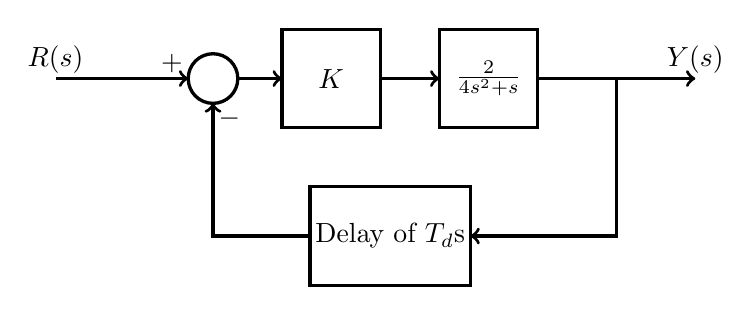
\begin{tikzpicture}[scale=1,inner sep=0pt,outer sep=0pt,very thick,
sysblock/.style={draw,rectangle,inner sep=2pt,minimum width=1.25cm,minimum height=1.25cm,very thick}]
\draw (2,0) node[draw,circle] (sum1) {$\rule{0pt}{18pt}$};
\draw (3.5,0) node[sysblock] (K) {$K$};
\draw (5.5,0) node[sysblock] (G) {$\frac{2}{4s^2+s}$};
\draw (4.25,-2) node[sysblock] (D) {Delay of $T_{d}$s};
\draw[->] (0,0) node[above=2pt] {$R(s)$} -- (sum1.180) node[above left=2pt] {$+$};
\draw[->] (sum1.0) --  (K);
\draw[->] (K) -- (G);
\draw[->] (G.0) -- ++(2,0) node[above=2pt] {$Y(s)$};
\draw[->] (G.0) ++(1,0) |- (D.0);
\draw[->] (D.180)  -| (sum1.-90) node[below right=2pt] {$-$};
\end{tikzpicture}
\end{center}
In the following, Let $K=1$. 
\begin{enumerate}[(a)]
\item Assuming $T_{d}=0$, use the linear approximation rules to sketch by hand the Bode plot for $KG(s)$, and using this, sketch by hand the Nyquist plot
\item From your Bode plot sketch, estimate the phase and gain margins for the feedback system
\item Determine the maximum delay $T_{d}$ that can be tolerated before the feedback loop becomes unstable. 
\end{enumerate}
